% --------------------------------------------------------------
% This is all preamble stuff that you don't have to worry about.
% Head down to where it says "Start here"
% --------------------------------------------------------------
 
\documentclass[12pt]{article}
 
\usepackage[margin=1in]{geometry}
\usepackage{amsmath,amsthm,amssymb}
\usepackage{graphicx} % Add this in the preamble if not already included
\usepackage{listings}
\usepackage{xcolor}
\usepackage{float}
\usepackage{url}
\lstset{
    basicstyle=\ttfamily\small,
    keywordstyle=\color{blue}\bfseries,
    commentstyle=\color{green!60!black},
    stringstyle=\color{orange},
    showstringspaces=false,
    breaklines=true,
    frame=single,
    numbers=left,
    numberstyle=\tiny,
    captionpos=b
}

\newcommand{\N}{\mathbb{N}}
\newcommand{\Z}{\mathbb{Z}}
 
\newenvironment{theorem}[2][Theorem]{\begin{trivlist}
\item[\hskip \labelsep {\bfseries #1}\hskip \labelsep {\bfseries #2.}]}{\end{trivlist}}
\newenvironment{lemma}[2][Lemma]{\begin{trivlist}
\item[\hskip \labelsep {\bfseries #1}\hskip \labelsep {\bfseries #2.}]}{\end{trivlist}}
\newenvironment{exercise}[2][Exercise]{\begin{trivlist}
\item[\hskip \labelsep {\bfseries #1}\hskip \labelsep {\bfseries #2.}]}{\end{trivlist}}
\newenvironment{problem}[2][Problem]{\begin{trivlist}
\item[\hskip \labelsep {\bfseries #1}\hskip \labelsep {\bfseries #2.}]}{\end{trivlist}}
\newenvironment{question}[2][Question]{\begin{trivlist}
\item[\hskip \labelsep {\bfseries #1}\hskip \labelsep {\bfseries #2.}]}{\end{trivlist}}
\newenvironment{corollary}[2][Corollary]{\begin{trivlist}
\item[\hskip \labelsep {\bfseries #1}\hskip \labelsep {\bfseries #2.}]}{\end{trivlist}}

\newenvironment{solution}{\begin{proof}[Solution]}{\end{proof}}
 
\begin{document}
 
% --------------------------------------------------------------
%                         Start here
% --------------------------------------------------------------
 
\title{Extra Credit Programming Assignment - GitHub Issue Resolution}%replace X with the appropriate number
\author{Rohit Reddy Musukudabbidi\\ %replace with your name
Web Technologies - 01 (Fall 2024)} %if necessary, replace with your course title
 
\maketitle
 
\section*{1. Introduction}

The \textbf{CSRankings React Native} project aimed to create a robust, mobile-optimized version of the \textit{CSRankings} website, known for ranking computer science institutions based on faculty research contributions. The existing web version, while functional, lacked usability and responsiveness on mobile devices. This necessitated a transition to a React Native application to enhance user experience and make the rankings more accessible to a global audience using Android and iOS platforms.

\bigskip
This project was guided by a clear objective: to replicate the core functionality and dynamic features of the \textit{CSRankings} website, such as filtering institutions by research areas, visualizing publication data, and providing detailed faculty profiles. The mobile application had to be intuitive, visually appealing, and efficient while maintaining the integrity of the data and rankings.

\bigskip
React Native was chosen for its ability to build cross-platform applications using a single codebase, reducing development time and ensuring consistency across platforms. The project focused on creating interactive features, such as dynamic filters and charts, while ensuring smooth navigation and a responsive user interface. The process involved designing custom components, integrating data from JSON files, and leveraging libraries like \texttt{react-navigation} and \texttt{react-native-chart-kit} for navigation and visualization.

\bigskip
\section*{2. Project Objective}

The primary objectives of the \textbf{CSRankings React Native} project were as follows:

\begin{enumerate}
    \item \textbf{Improve Mobile Usability:} \\
    Develop a React Native application optimized for mobile platforms to address the usability challenges of the original \textit{CSRankings} website on smaller screens.
    
    \item \textbf{Seamless Cross-Platform Performance:} \\
    Ensure smooth and consistent performance across both Android and iOS devices.
    
    \item \textbf{Feature Replication:} \\
    Recreate all key features of the \textit{CSRankings} website, including rankings, filters, detailed institution pages, and research area visualizations.
    
    \item \textbf{Enhanced UI/UX:} \\
    Design a clean, modern, and intuitive user interface that maintains consistency with the original website while improving user engagement.
    
    \item \textbf{Interactive Functionalities:} \\
    Implement advanced features such as dynamic filters for research areas and real-time, interactive charts for publication data visualization.
\end{enumerate}

\bigskip
\section*{3. Requirements Analysis}

Based on the project brief, the application was designed to replicate the core functionality of the \textit{CSRankings} website while enhancing its usability for mobile devices. The key requirements identified for the application were as follows:

\begin{enumerate}
    \item \textbf{Homepage Listing Institutions:} \\
    A primary screen displaying institutions ranked based on publication data, similar to the original website, but optimized for smaller screens and touch navigation.
    
    \item \textbf{Dynamic Filters:} \\
    Interactive filters allowing users to narrow down rankings based on research areas such as Artificial Intelligence, Systems, Theory, and Interdisciplinary Areas.
    
    \item \textbf{Institution Detail Pages:} \\
    Dedicated pages for each institution providing detailed information, including faculty names, their research areas, and links to their academic profiles.
    
    \item \textbf{Charts for Data Visualization:} \\
    Interactive bar charts to dynamically visualize publication data for different research areas, enhancing user engagement and comprehension.
    
    \item \textbf{Cross-Platform Compatibility:} \\
    Seamless functionality and consistent UI/UX across both Android and iOS platforms to cater to a wide user base.
    
    \item \textbf{Modern Design and Performance Optimization:} \\
    Ensure the application delivers a smooth experience, with minimal load times and responsive interactions tailored for mobile devices.
\end{enumerate}

\bigskip
\section*{4. Technology Stack}

The project utilized the following technologies:

\begin{itemize}
    \item \textbf{React Native:} For cross-platform mobile development.
    \item \textbf{Expo:} To simplify the development, testing, and deployment process.
    \item \textbf{React Navigation:} For navigation and routing.
    \item \textbf{React Native Chart Kit:} For data visualization through charts.
    \item \textbf{Jest:} For writing and executing test cases.
    \item \textbf{GitHub:} For version control and collaboration.
    \item \textbf{VS Code:} As the primary code editor.
\end{itemize}

\bigskip
\section*{5. Development Process}
This section provides a detailed step-by-step explanation of the development process, starting from understanding the CSRankings concept and data structure to implementing the features and functionalities of the application.

\subsection*{5.1 Understanding CSRankings and Data Structure}

The first step involved thoroughly understanding the \textit{CSRankings} website, its purpose, and how it operates:

\subsubsection*{Concept of CSRankings}
\textit{CSRankings} is an interactive platform that ranks computer science institutions based on research publications in selective conferences. It is highly data-driven and focuses on categorizing institutions by research areas and their contributions.

\subsubsection*{Key Components of CSRankings}
\begin{itemize}
    \item \textbf{Institution Rankings:} Institutions are ranked based on the number of publications by their faculty.
    \item \textbf{Research Areas:} Publications are grouped into categories such as Artificial Intelligence, Systems, Theory, and Interdisciplinary Areas.
    \item \textbf{Faculty Details:} Each institution lists its faculty members, their research areas, and links to their academic profiles.
\end{itemize}

\subsubsection*{Understanding Data Sources}
\begin{itemize}
    \item \texttt{universities.json}: Provided the list of institutions.
    \item \texttt{rank.json}: Contained publication data linked to institutions.
    \item \texttt{subarea.json}: Defined the research areas and subcategories.
    \item \texttt{faculty.json}: Detailed the faculty members and their publication records.
\end{itemize}



\begin{figure}[h]
    \centering
    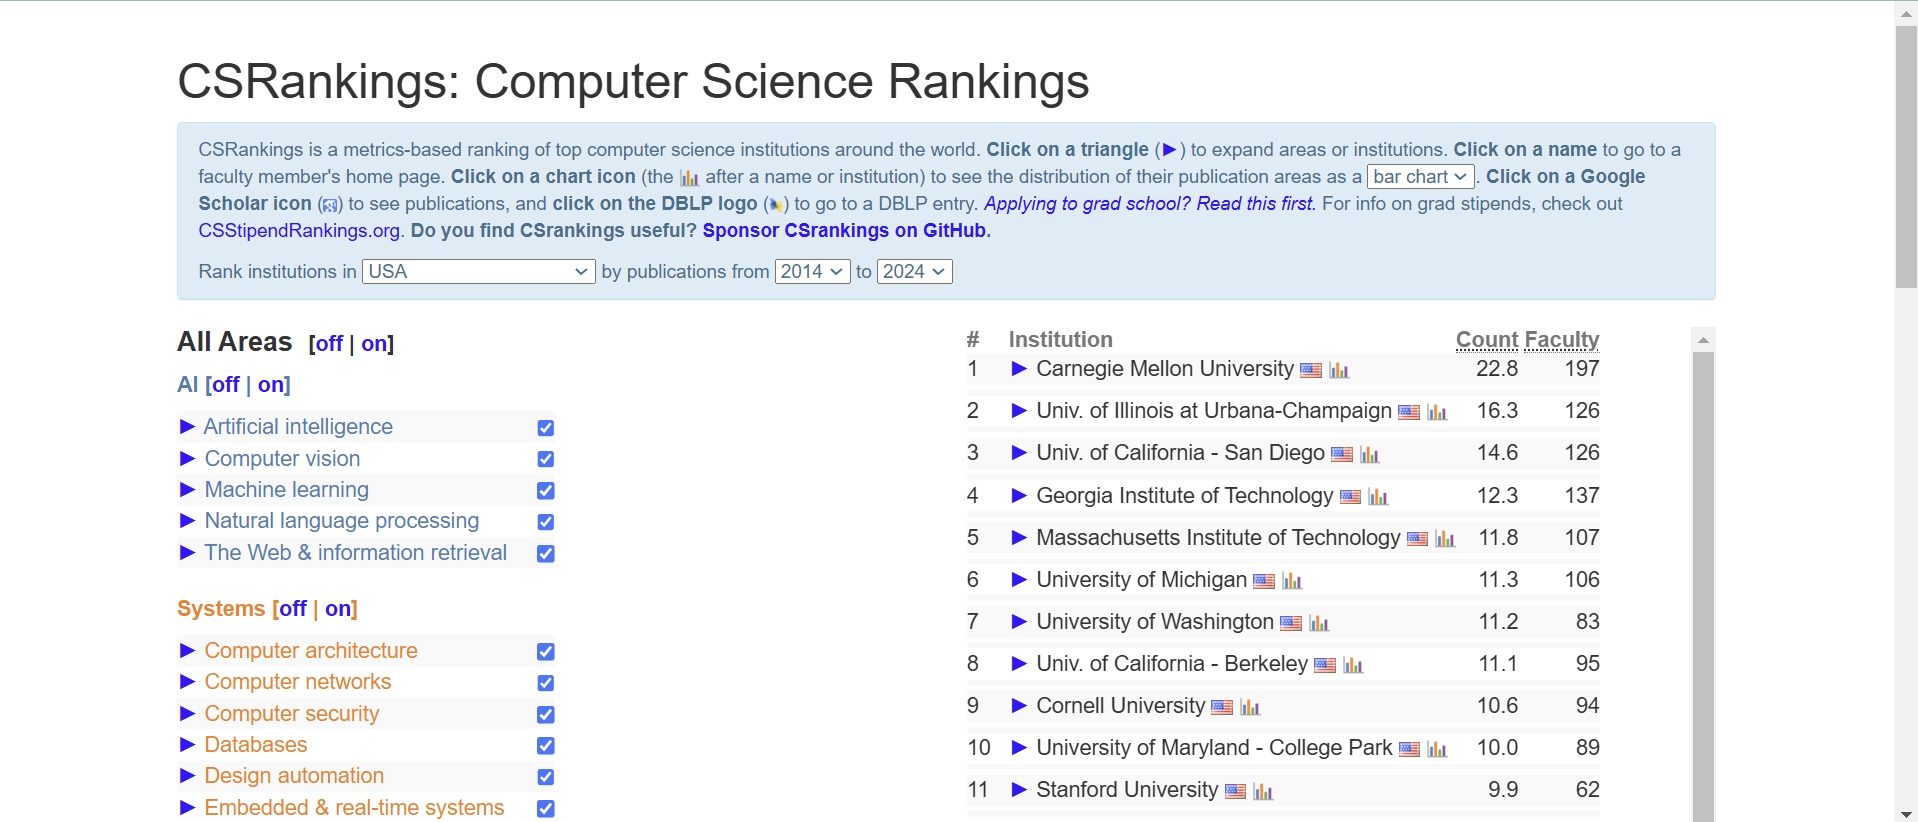
\includegraphics[width=\textwidth]{csr.png} % Replace with your image file
    \caption{CSRankings top institutions overview.}
    \label{fig:example_image}
\end{figure}

\begin{figure}[h]
    \centering
    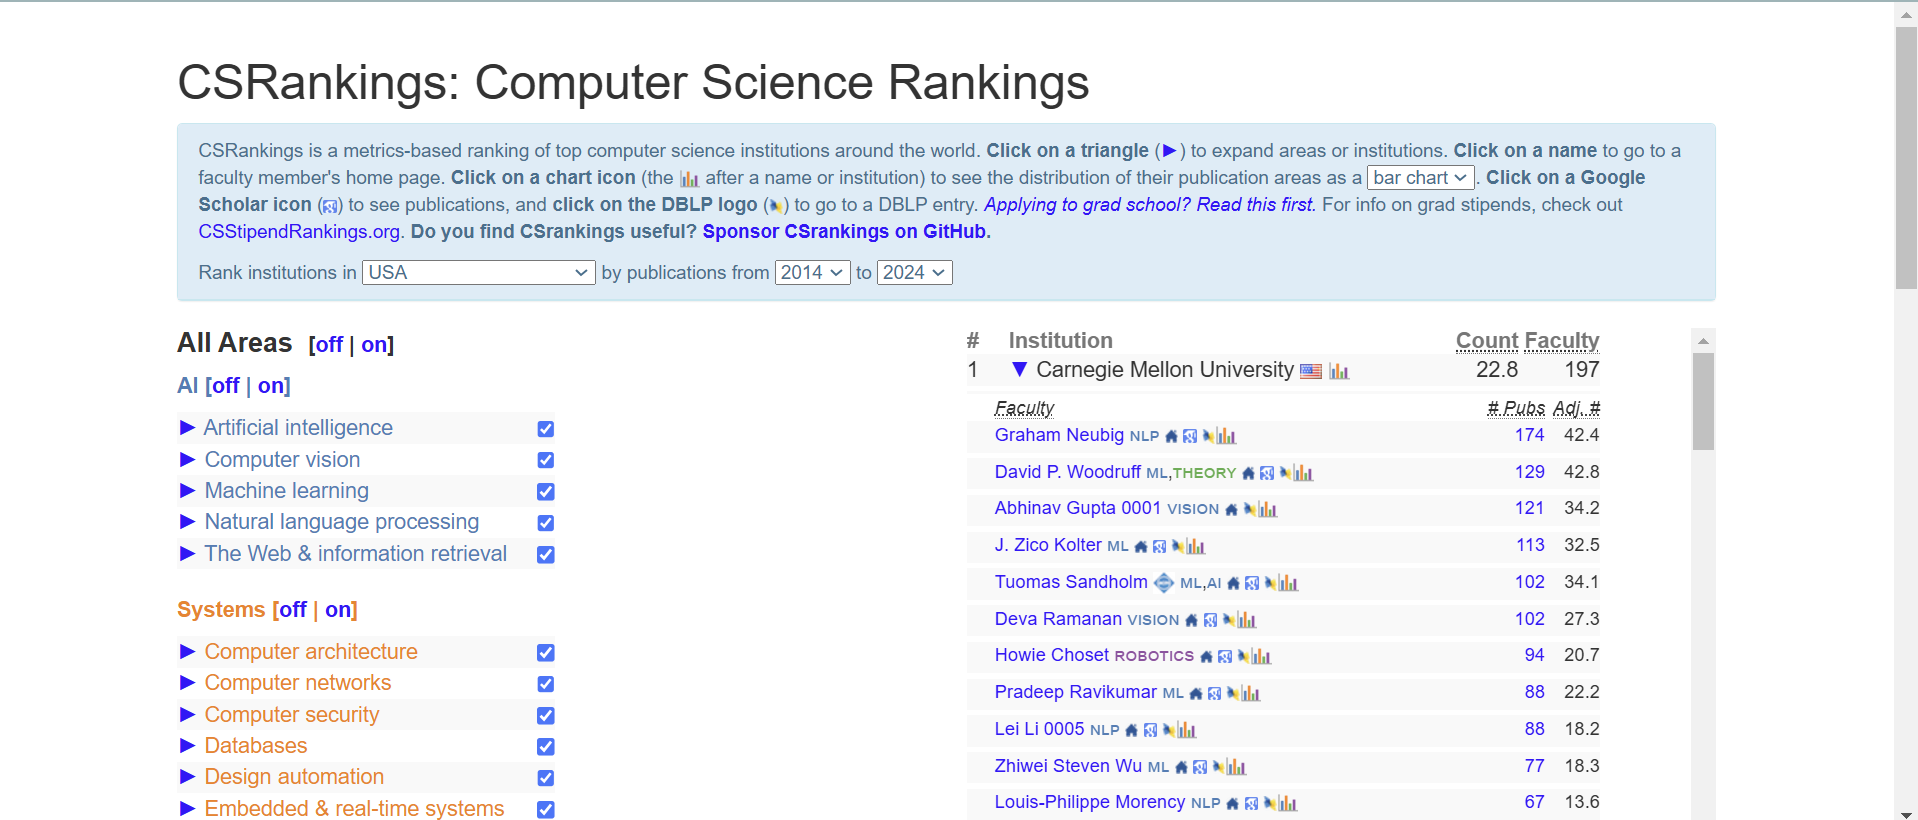
\includegraphics[width=\textwidth]{csr2.png} % Replace with your image file
    \caption{CSRankings platform highlighting Carnegie Mellon University and faculty details.}
    \label{fig:example_image}
\end{figure}

\subsection*{5.2 Setting Up the Project Environment}

\subsubsection*{Choosing the Framework}
\begin{itemize}
    \item \textbf{React Native:} Selected for its ability to create cross-platform mobile applications using a single codebase.
    \item \textbf{Expo:} Used for easier setup and debugging during development.
\end{itemize}

\subsubsection*{Project Initialization}
\begin{itemize}
    \item Project initialized using the following command:
    \begin{verbatim}
    npx create-expo-app CSRanking
    \end{verbatim}
    \item Installed the required dependencies:
    \begin{itemize}
        \item \texttt{react-native-chart-kit} for charts.
        \item \texttt{react-navigation} for multi-screen navigation.
        \item \texttt{@react-native-picker/picker} for dropdowns.
        \item \texttt{react-native-vector-icons} for UI icons.
    \end{itemize}
\end{itemize}

\subsubsection*{Project Folder Structure}
\begin{itemize}
    \item Organized the project with directories for screens, components, and data:
    \begin{itemize}
        \item \textbf{Components:} \texttt{HomeScreen}, \texttt{InstitutionDetails}, \texttt{ChartScreen}, \texttt{AboutScreen}, \texttt{Navigator}.
        \item \textbf{Data:} Static JSON files simulating backend data.
        \item \textbf{\_tests\_:} Jest test files.
    \end{itemize}
\end{itemize}

\bigskip
\subsection*{5.3 Data Integration}

\subsubsection*{Creating Data}
\begin{itemize}
    \item Created JSON files (\texttt{universities.json}, \texttt{rank.json}, \texttt{subarea.json}, \texttt{faculty.json}) for the project.
    \item Used \texttt{useEffect} hooks to simulate asynchronous data loading.
\end{itemize}

\begin{figure}[H]
    \centering
    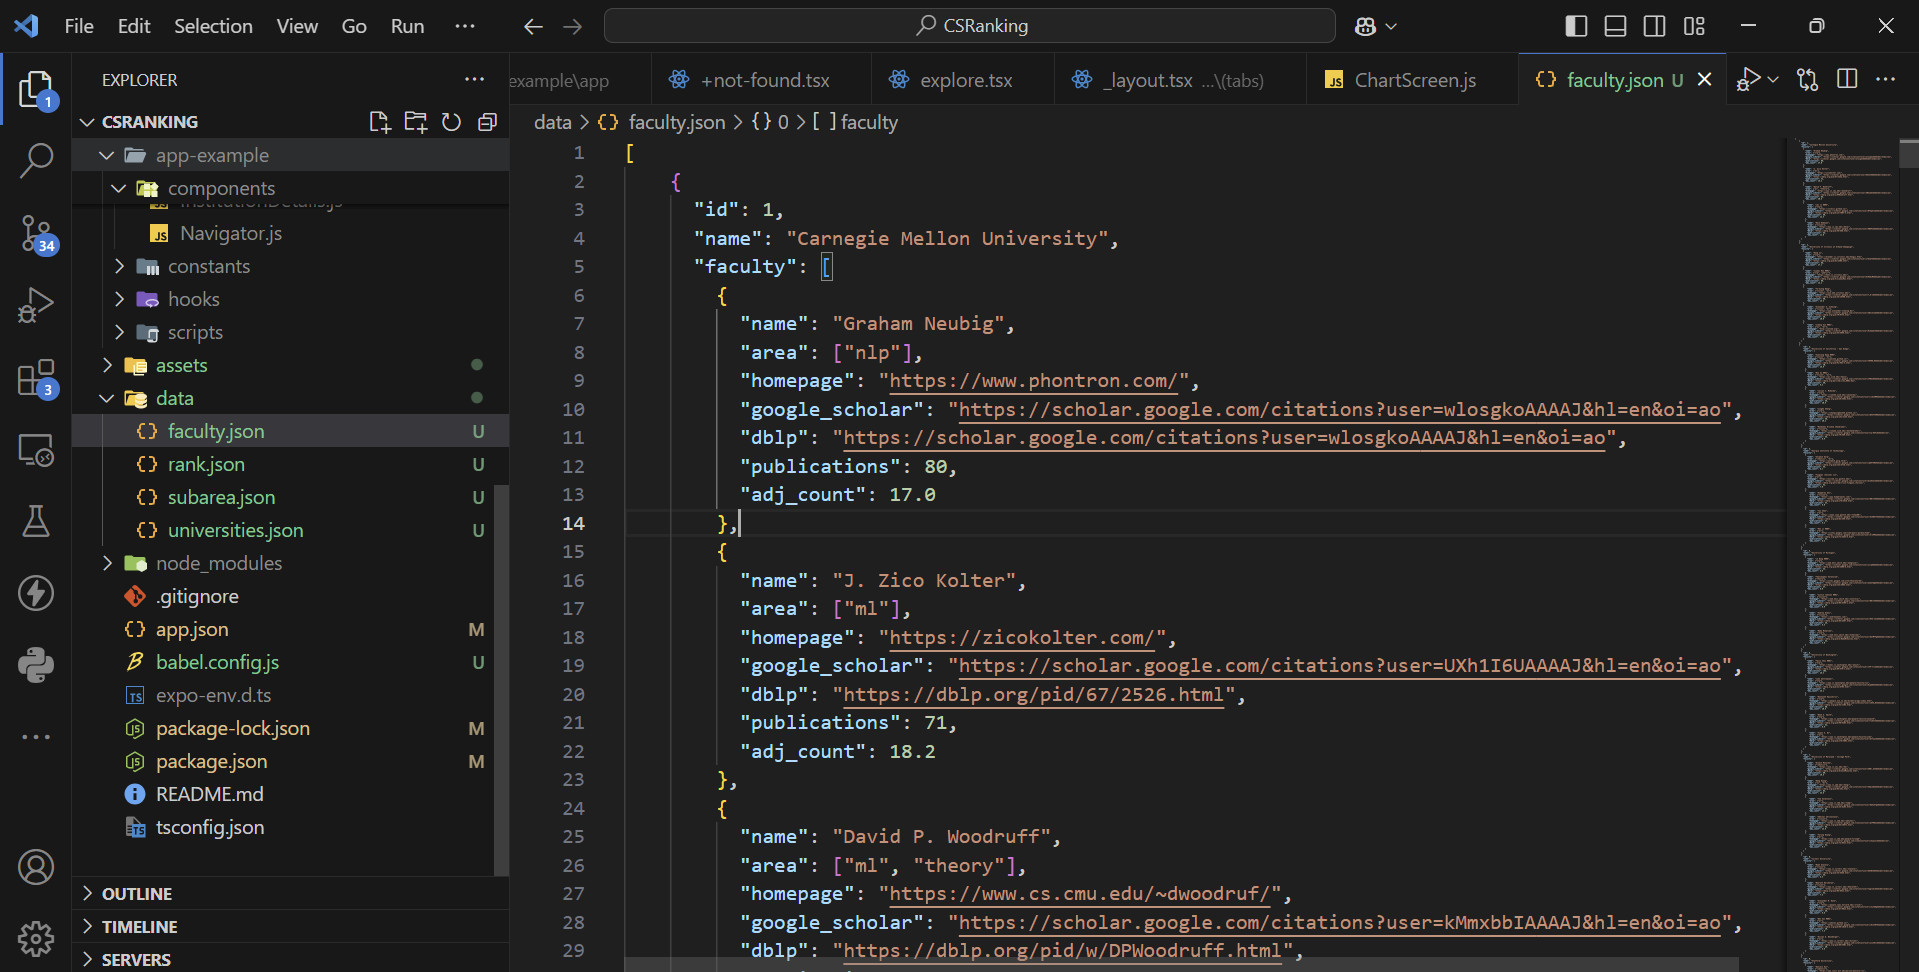
\includegraphics[width=\textwidth]{json1.png} % Replace with your image file
    \caption{faculty.json.}
    \label{fig:example_image}
\end{figure}

\begin{figure}[H]
    \centering
    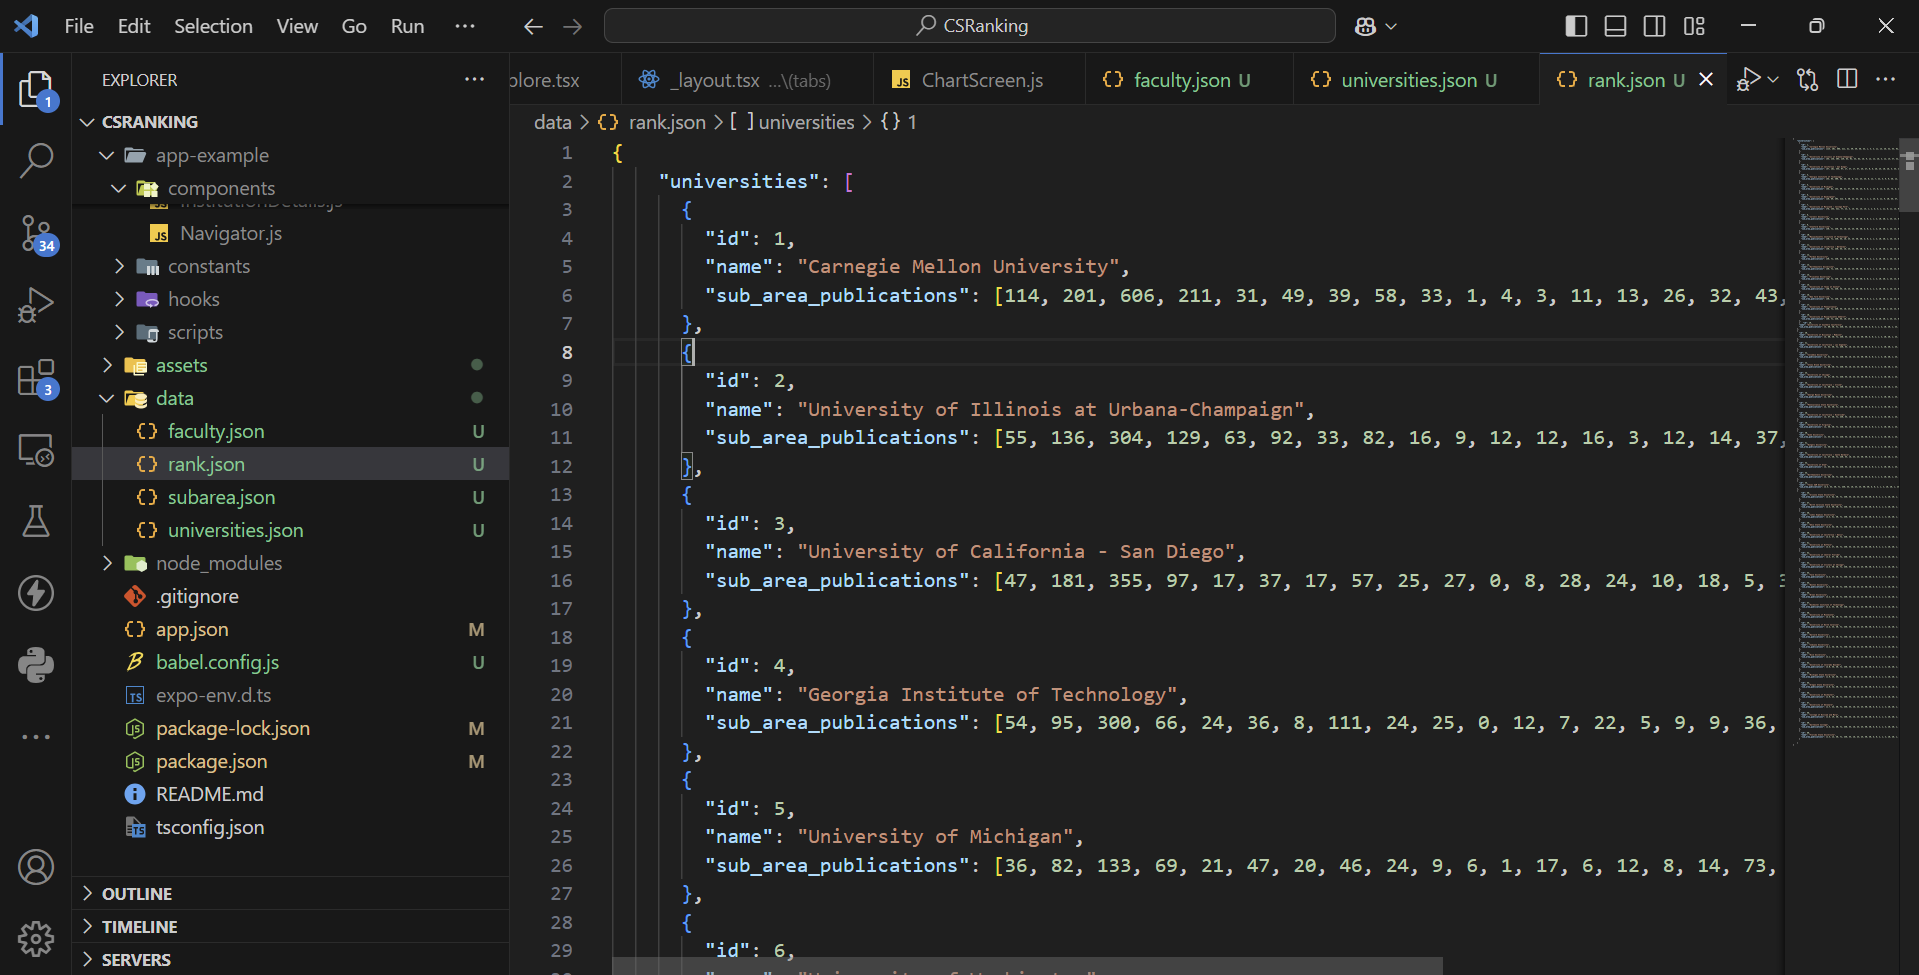
\includegraphics[width=\textwidth]{json2.png} % Replace with your image file
    \caption{rank.json.}
    \label{fig:example_image}
\end{figure}

\begin{figure}[H]
    \centering
    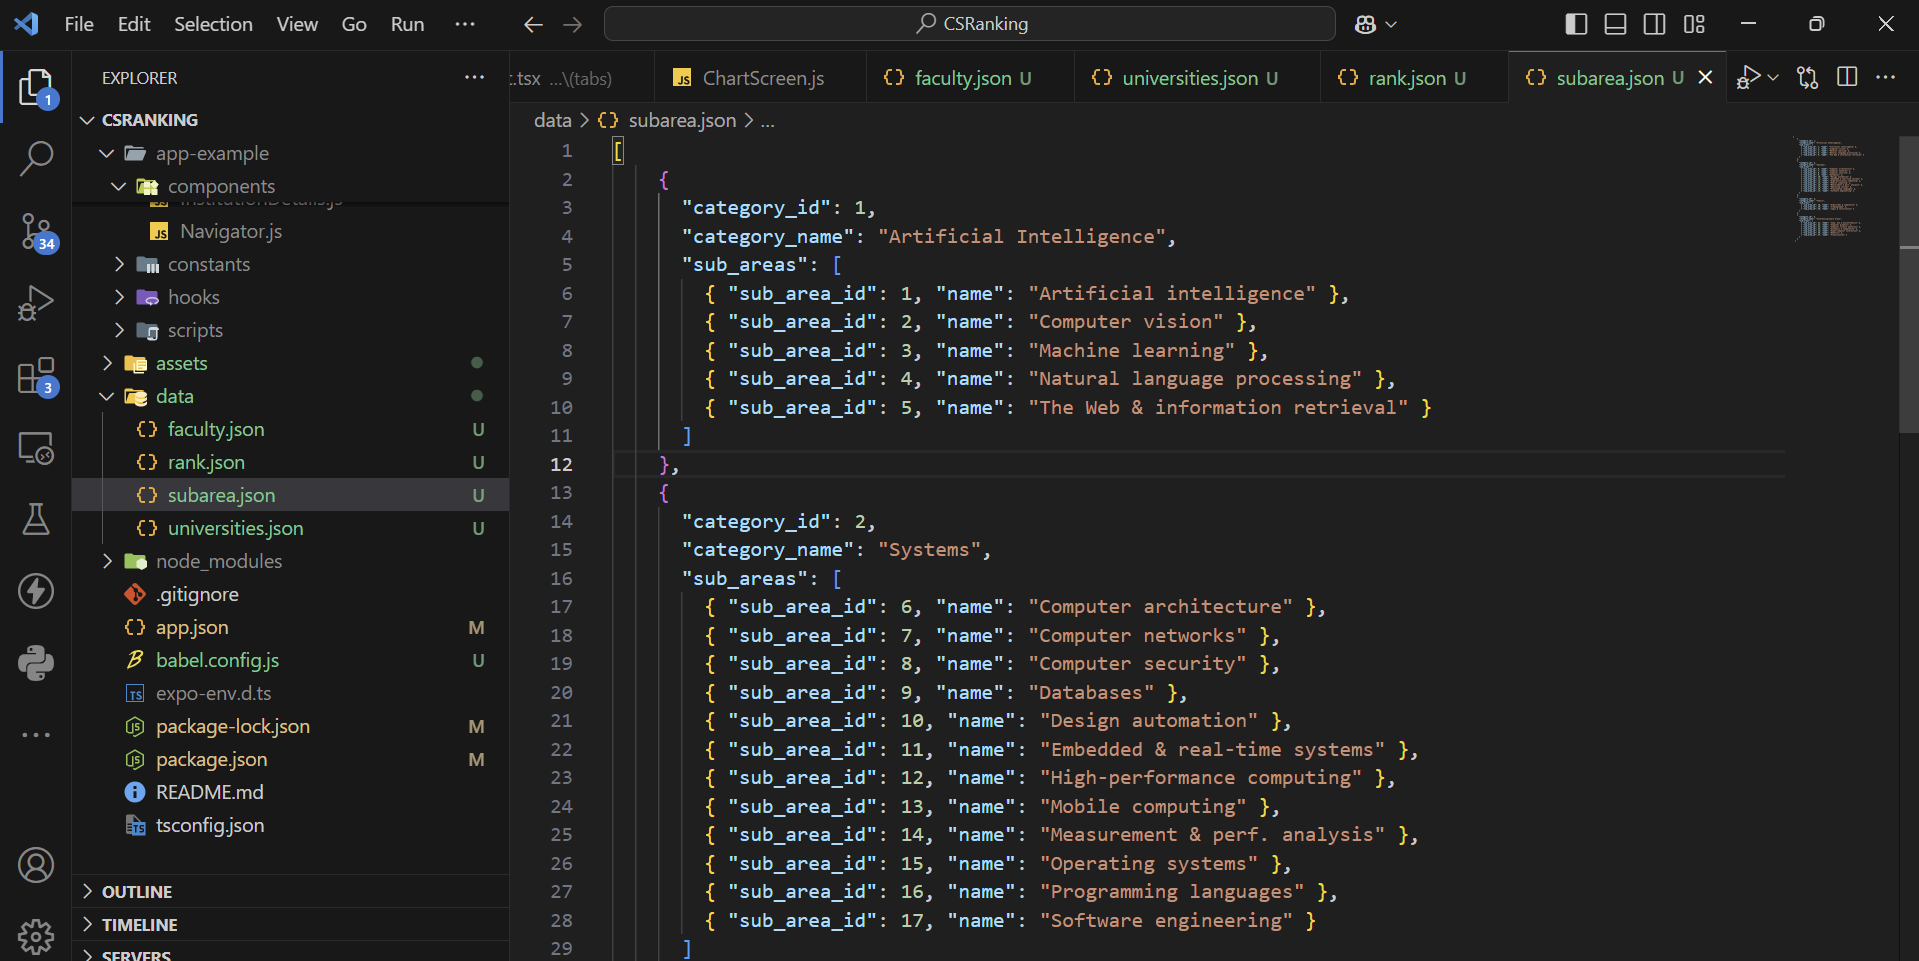
\includegraphics[width=\textwidth]{json3.png} % Replace with your image file
    \caption{subarea.json.}
    \label{fig:example_image}
\end{figure}

\begin{figure}[H]
    \centering
    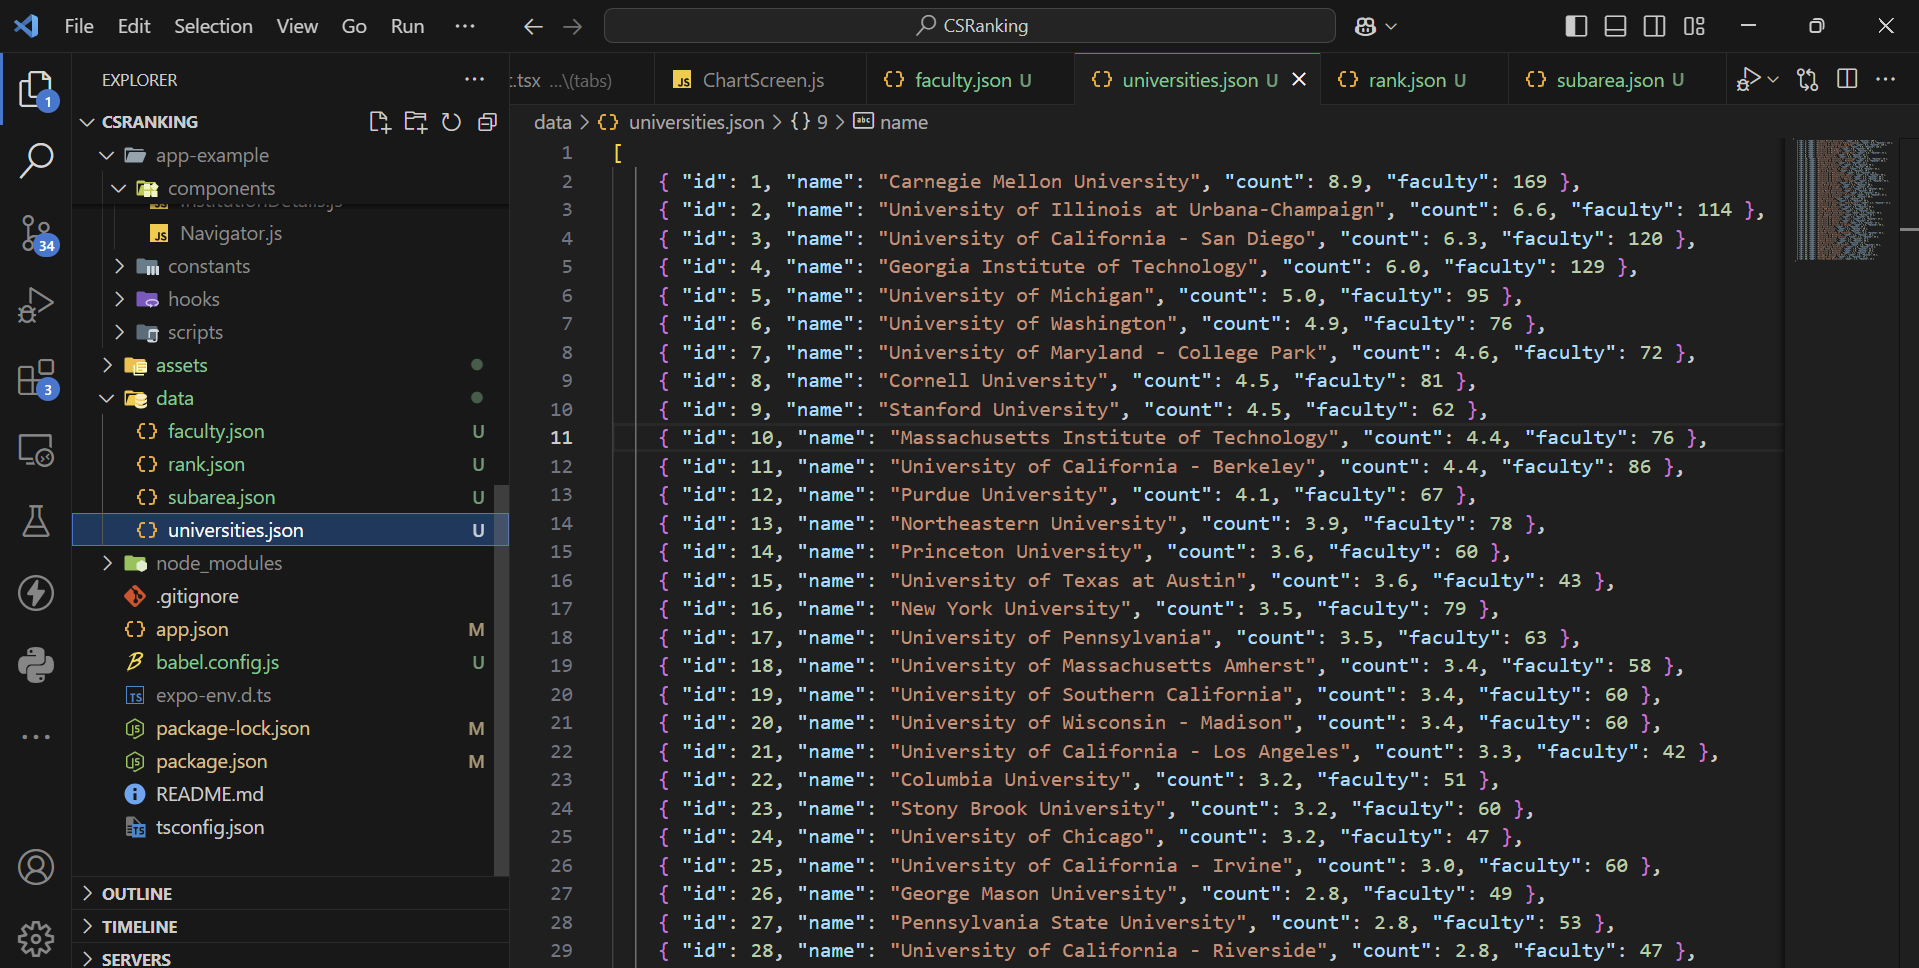
\includegraphics[width=\textwidth]{json4.png} % Replace with your image file
    \caption{universities.json.}
    \label{fig:example_image}
\end{figure}

\subsubsection*{Linking Data}
\begin{itemize}
    \item Merged \texttt{universities.json} with \texttt{rank.json} to associate publication counts with institutions.
    \item Linked \texttt{faculty.json} to each institution to provide faculty details.
\end{itemize}

\begin{lstlisting}[language=JavaScript, caption={Dynamic Data Integration with \texttt{useEffect}}, label={lst:useEffectDataIntegration}]
useEffect(() => {
    setTimeout(() => {
        const mergedData = data.map((university) => {
            const rankInfo = rankData.universities.find((rank) => rank.name === university.name);
            return {
                ...university,
                sub_area_publications: rankInfo ? rankInfo.sub_area_publications : [],
            };
        });
        setInstitutions(mergedData);
        setLoading(false);
    }, 1000);
}, []);
\end{lstlisting}


\subsubsection*{5.4 Dynamic Data Handling}
\begin{itemize}
    \item Created utility functions to filter and sort data dynamically based on user interactions.
    \item Used React state (\texttt{useState}) to manage filters, search input, and selected institution details.
\end{itemize}

\subsection*{5.5 Frontend Development}

\subsubsection*{5.5.1 Homepage Development}
\begin{itemize}
    \item \textbf{Institution List:}
    \begin{itemize}
        \item Displayed a ranked list of institutions dynamically.
        \item Used \texttt{FlatList} for efficient rendering of large datasets.
    \end{itemize}

    \item \textbf{Search Bar:}
    \begin{itemize}
        \item Added a \texttt{TextInput} component for users to search institutions by name.
        \item Dynamically filtered the institution list based on search input.
    \end{itemize}
    \begin{lstlisting}[language=JavaScript, caption={Filtering Data by Search Term}, label={lst:filteredData}]
const filteredData = getFilteredData().filter((item) =>
    item.name.toLowerCase().includes(search.toLowerCase())
);
\end{lstlisting}

    \item \textbf{Filters:}
    \begin{itemize}
        \item Created a filter modal to toggle between research areas (AI, Systems, Theory, etc.).
        \item Updated the institution ranking based on selected filters.
        \item Used state to track active filters.
    \end{itemize}
\end{itemize}
\begin{lstlisting}[language=JavaScript, caption={Filtering Data by Sub-Areas}, label={lst:getFilteredData}]
const getFilteredData = () => {
    if (filters.allAreas) return institutions;

    const { selectedSubAreas } = filters;
    if (selectedSubAreas.length === 0) return institutions;

    return institutions
      .map((inst) => {
        const totalPublications = selectedSubAreas.reduce((sum, subAreaId) => {
          return sum + (inst.sub_area_publications[subAreaId - 1] || 0);
        }, 0);
        return { ...inst, totalPublications };
      })
      .sort((a, b) => b.totalPublications - a.totalPublications);
};
\end{lstlisting}

\begin{figure}[H]
    \centering
    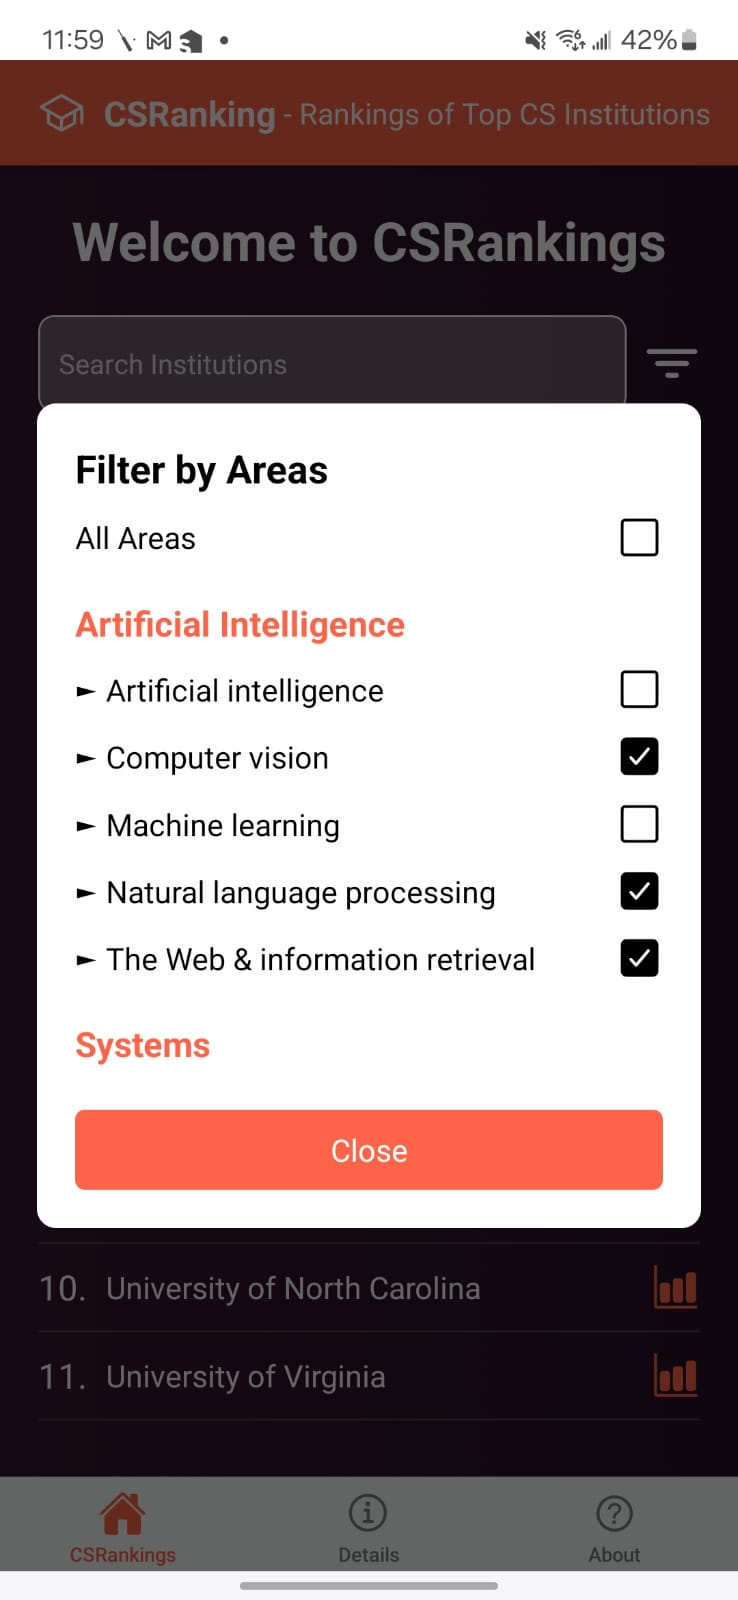
\includegraphics[width=0.3\textwidth, height=0.4\textheight]{filter.jpg} % Adjust width and height as needed
    \caption{Filters.}
    \label{fig:example_image}
\end{figure}

\subsubsection*{5.5.2 Institution Details Page}
\begin{itemize}
    \item Displayed detailed information for the selected institution:
    \begin{itemize}
        \item Faculty names, research areas, and publication statistics.
        \item External links to Google Scholar, DBLP, and personal homepages.
    \end{itemize}
    \item Integrated \texttt{react-native-vector-icons} for navigation buttons and styling.
\end{itemize}
\begin{lstlisting}[language=JavaScript, caption={Fetching Faculty Data based on Institution}, label={lst:useEffectFaculty}]
useEffect(() => {
    if (institution) {
        const institutionDetails = facultyData.find(
            (inst) => inst.name === institution.name
        );
        setFacultyList(institutionDetails ? institutionDetails.faculty : []);
    }
}, [institution]);
\end{lstlisting}

\begin{figure}[H]
    \centering
    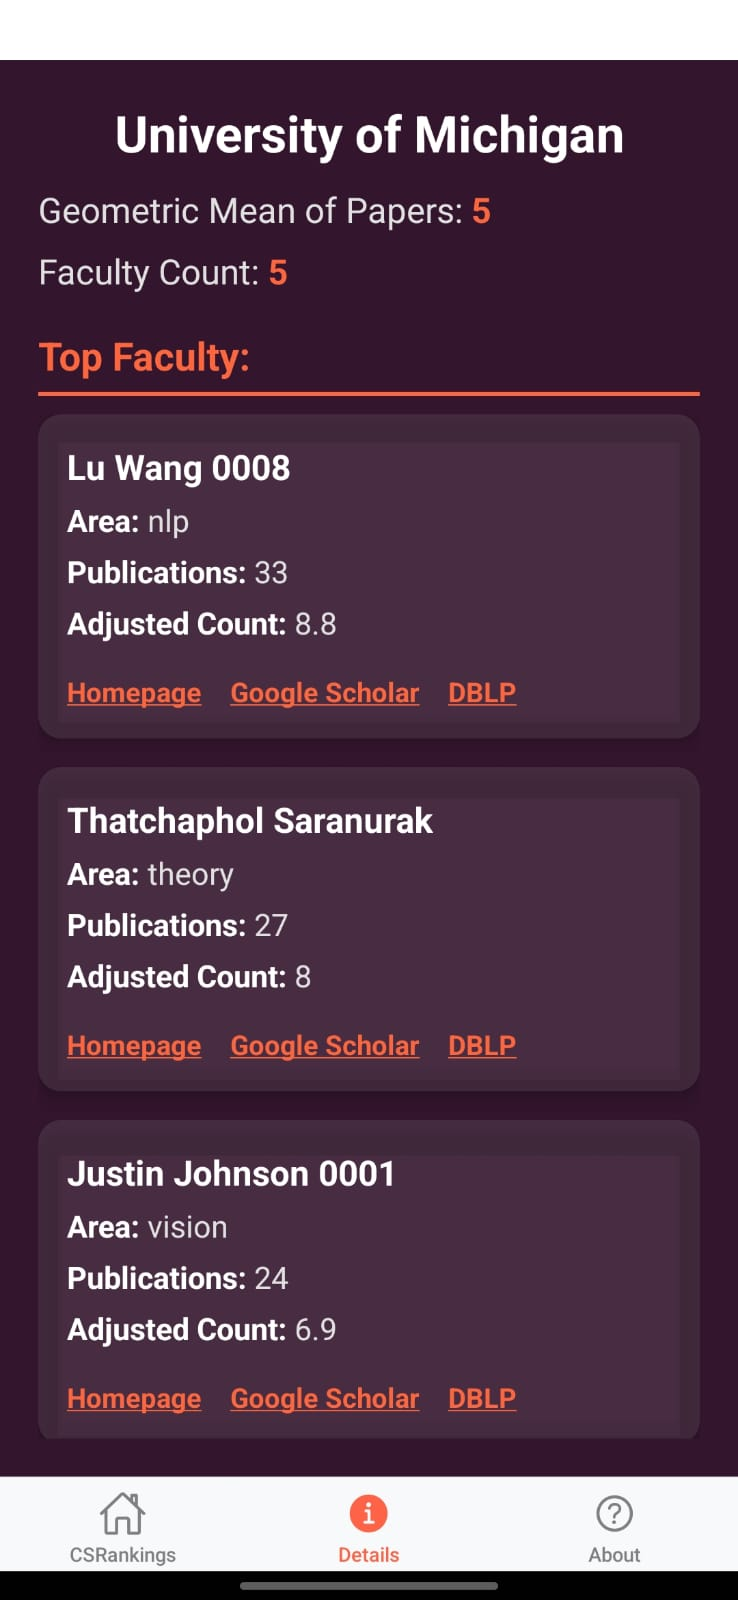
\includegraphics[width=0.3\textwidth, height=0.5\textheight]{institution.jpg} % Adjust width and height as needed
    \caption{Institution Page.}
    \label{fig:example_image}
\end{figure}


\clearpage
\subsubsection*{5.5.3 Chart Integration}
\begin{itemize}
    \item Added interactive bar charts using \texttt{react-native-chart-kit}.
    \item Dynamically displayed publication data for selected research areas.
    \item Enabled horizontal scrolling for charts with long labels.
    \item Included a legend to decode chart abbreviations.
\end{itemize}

\begin{lstlisting}[language=JavaScript, caption={BarChart Integration within ScrollView}, label={lst:BarChart}]
<ScrollView horizontal>
    <BarChart
        data={{
            labels,
            datasets: [{ data: chartData }],
        }}
        width={Math.max(labels.length * 80, Dimensions.get('window').width - 20)}
        height={400}
        yAxisLabel=""
        chartConfig={{
            backgroundColor: '#1cc910',
            backgroundGradientFrom: '#eff3ff',
            backgroundGradientTo: '#efefef',
            decimalPlaces: 0,
            color: (opacity = 1) => `rgba(0, 0, 0, ${opacity})`,
            labelColor: (opacity = 1) => `rgba(0, 0, 0, ${opacity})`,
            barPercentage: 0.8,
            useShadowColorFromDataset: false,
        }}
        style={styles.chartWithPadding}
        verticalLabelRotation={0}
        fromZero
        showValuesOnTopOfBars={true}
        onDataPointClick={(data) => handleBarPress(data.index)}
    />
</ScrollView>
\end{lstlisting}

\begin{figure}[H]
    \centering
    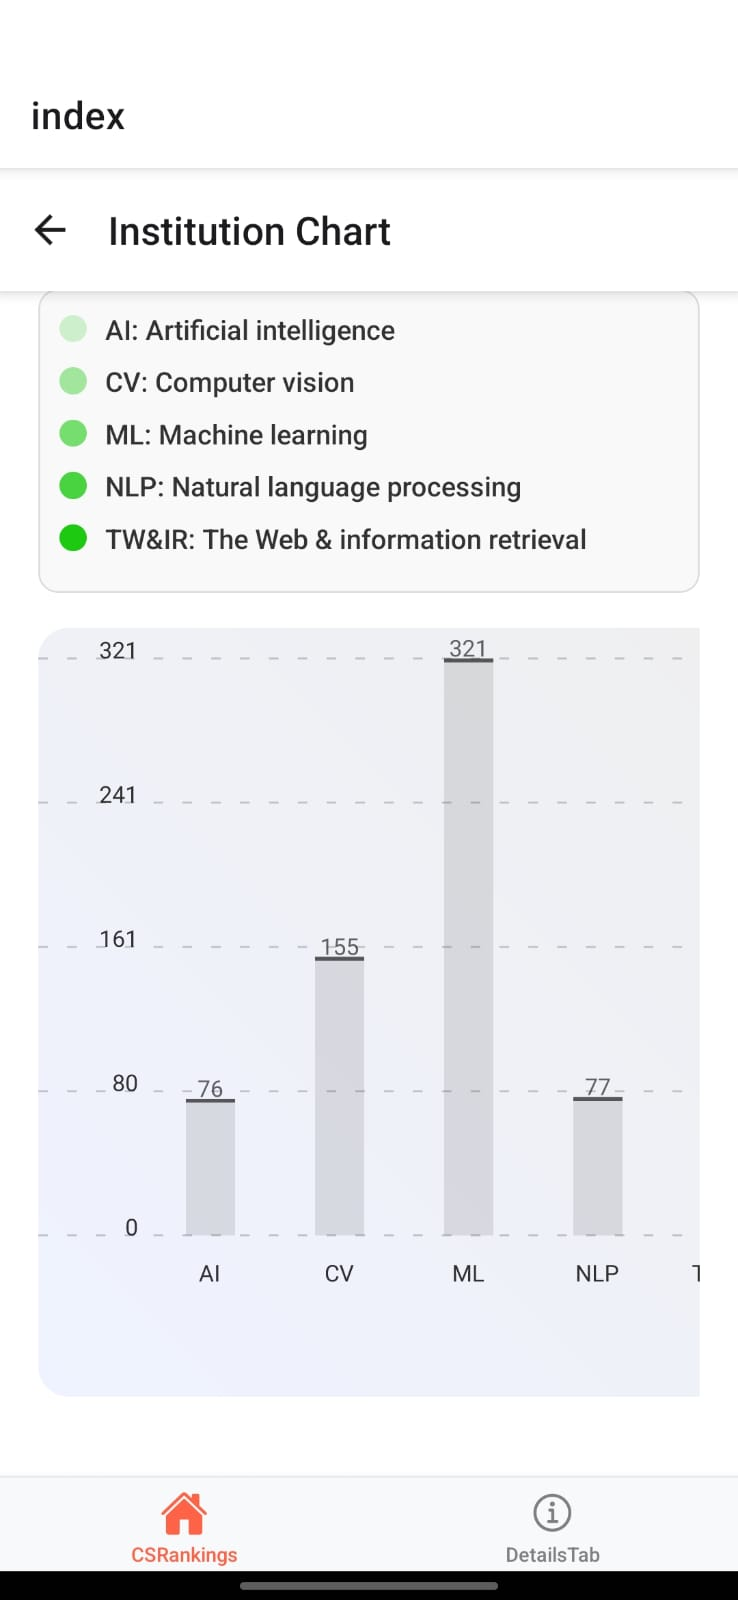
\includegraphics[width=0.3\textwidth, height=0.4\textheight]{chart1.jpg} % Adjust width and height as needed
    \caption{Chart Screen Page.}
    \label{fig:example_image}
\end{figure}
\begin{figure}[H]
    \centering
    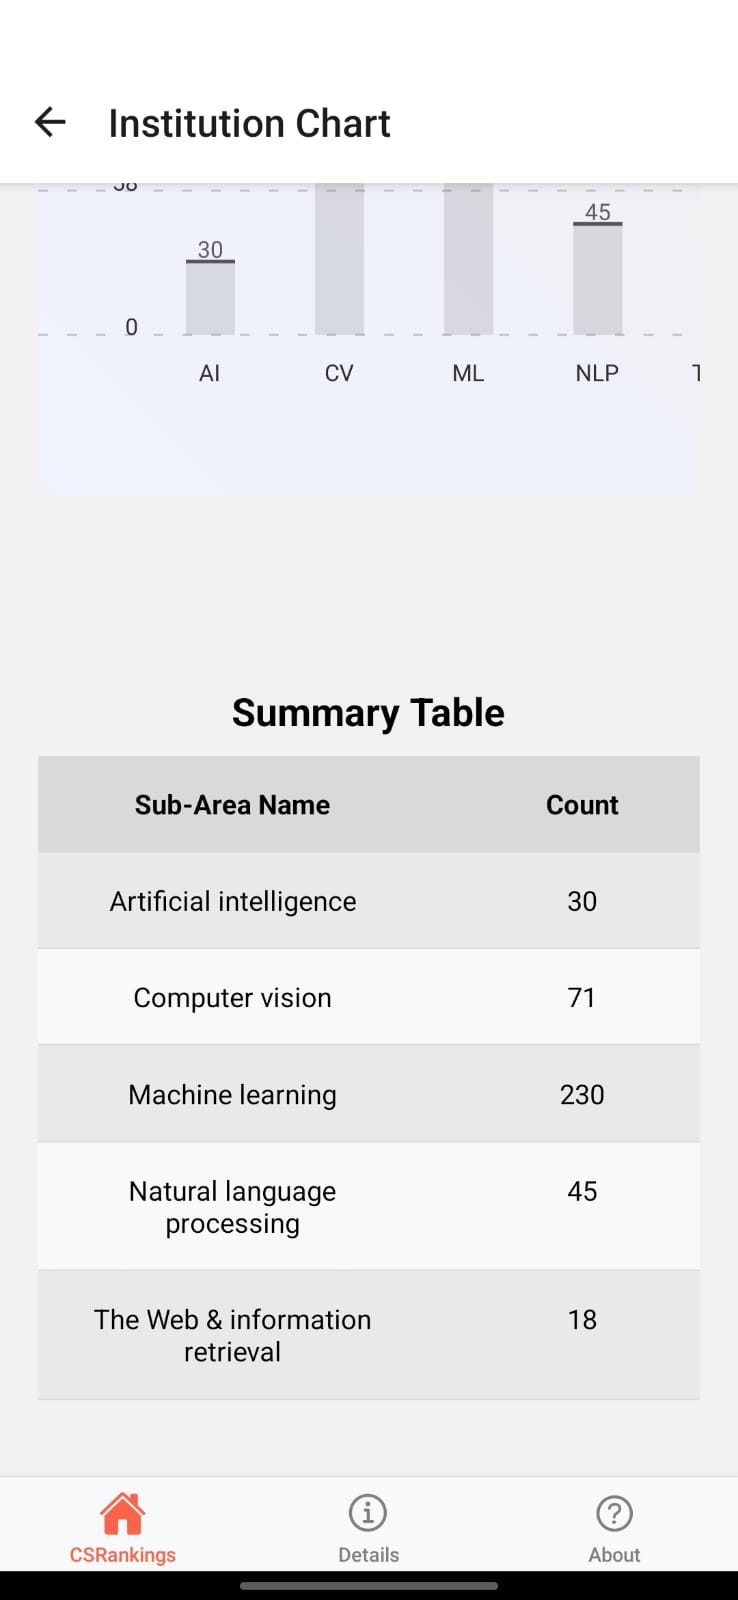
\includegraphics[width=0.3\textwidth, height=0.4\textheight]{chart2.jpg} % Adjust width and height as needed
    \caption{Chart Screen Page.}
    \label{fig:example_image}
\end{figure}



\clearpage
\subsubsection*{5.5.4 About Page}
\begin{itemize}
    \item Provided an overview of CSRankings, including its purpose and methodology.
    \item Highlighted mentions of CSRankings by renowned institutions and individuals.
    \item Included clickable links to GitHub, DBLP, FAQs, and licensing details.
    \item Integrated a clickable YouTube thumbnail linking to an introductory video.
    \item Styled with responsive design for mobile devices using \texttt{ScrollView} and consistent fonts and colors.
\end{itemize}
\begin{lstlisting}[language=JavaScript, caption={About CSRankings View}, label={lst:AboutCSRankings}]
<View style={styles.container}>
  <ScrollView contentContainerStyle={styles.contentContainer}>
    <Text style={styles.title}>About CSRankings</Text>
    <Text style={styles.description}>
      This ranking is designed to identify institutions and faculty actively engaged in research across a number of
      areas of computer science, based on the number of publications by faculty that have appeared at the most
      selective conferences in each area of computer science (see the FAQ for more details).
    </Text>

    <Text style={styles.description}>
      We gratefully acknowledge the generous support of our sponsors, including Stony Brook University. Sponsor CSrankings.
    </Text>

    <TouchableOpacity onPress={() => Linking.openURL('https://www.youtube.com/watch?v=hOSl3xPmHiQ&t=232s')}>
      <Image
        style={styles.videoImage}
        source={{
          uri: 'https://img.youtube.com/vi/hOSl3xPmHiQ/0.jpg',
        }}
      />
      <Text style={styles.videoText}>Click the image above to watch the introduction video on YouTube.</Text>
    </TouchableOpacity>

  </ScrollView>
</View>
\end{lstlisting}

\begin{figure}[H]
    \centering
    
\includegraphics[width=0.3\textwidth, height=0.5\textheight]{about.jpg} % Adjust width and height as needed
    \caption{About Page.}
    \label{fig:example_image}
\end{figure}


\subsection*{5.5.5 Navigator Component}
The Navigator component is the central navigation structure of the CSRankings app. It combines a Bottom Tab Navigator for main sections and a Stack Navigator for deeper navigation, enabling seamless transitions between screens.

\begin{lstlisting}[language=JavaScript, caption={Navigator Component Implementation}, label={lst:NavigatorComponent}]
<Tab.Navigator
  screenOptions={({ route }) => ({
    headerShown: false,
    tabBarStyle: { backgroundColor: '#f8f9fa' },
    tabBarIcon: ({ focused, color, size }) => {
      let iconName;
      if (route.name === 'HomeTab') iconName = focused ? 'home' : 'home-outline';
      else if (route.name === 'DetailsTab') iconName = focused ? 'information-circle' : 'information-circle-outline';
      else if (route.name === 'AboutTab') iconName = focused ? 'help-circle' : 'help-circle-outline';
      return <Ionicons name={iconName} size={size} color={color} />;
    },
    tabBarActiveTintColor: 'tomato',
    tabBarInactiveTintColor: 'gray',
  })}
>
  <Tab.Screen name="HomeTab" component={HomeStack} options={{ title: 'CSRankings' }} />
  <Tab.Screen name="DetailsTab" component={InstitutionDetails} options={{ title: 'Details' }} />
  <Tab.Screen name="AboutTab" component={AboutScreen} options={{ title: 'About' }} />
</Tab.Navigator>
\end{lstlisting}

\subsubsection*{Component Details}
\textbf{HomeStack:}
\begin{itemize}
    \item Implements a Stack Navigator to manage navigation between:
    \begin{itemize}
        \item \textbf{Home Screen:} Displays the list of institutions and rankings.
        \item \textbf{Chart Screen:} Visualizes publication data with interactive bar charts.
    \end{itemize}
    \item \textbf{Key Configurations:}
    \begin{itemize}
        \item \texttt{headerShown: false}: Ensures no header is displayed for the Home screen for a cleaner UI.
        \item \texttt{Dynamic Titles:} Displays a descriptive title for the Chart screen.
    \end{itemize}
\end{itemize}

\textbf{Tab.Navigator:}
\begin{itemize}
    \item Implements a Bottom Tab Navigator for the main sections:
    \begin{itemize}
        \item \textbf{HomeTab:} Navigates to the Home Stack.
        \item \textbf{DetailsTab:} Directly displays the Institution Details screen.
        \item \textbf{AboutTab:} Displays the About screen with project information.
    \end{itemize}
    \item \textbf{Dynamic Icon Handling:}
    \begin{itemize}
        \item Uses \texttt{react-native-vector-icons/Ionicons} for tab icons.
        \item Icons change based on focus (e.g., \texttt{home} vs \texttt{home-outline}).
    \end{itemize}
    \item \textbf{Styling:}
    \begin{itemize}
        \item \textbf{Active Tab:} Highlighted with a tomato color.
        \item \textbf{Inactive Tab:} Shown in gray.
        \item Background styled with light gray.
    \end{itemize}
\end{itemize}

\textbf{Key Functionalities:}
\begin{itemize}
    \item \textbf{Responsive Navigation:} Works seamlessly across Android and iOS.
    \item \textbf{Modular Design:}
    \begin{itemize}
        \item Separates the navigation logic for clarity and reusability.
        \item Ensures easy updates and maintenance.
    \end{itemize}
\end{itemize}

\begin{figure}[H]
    \centering
    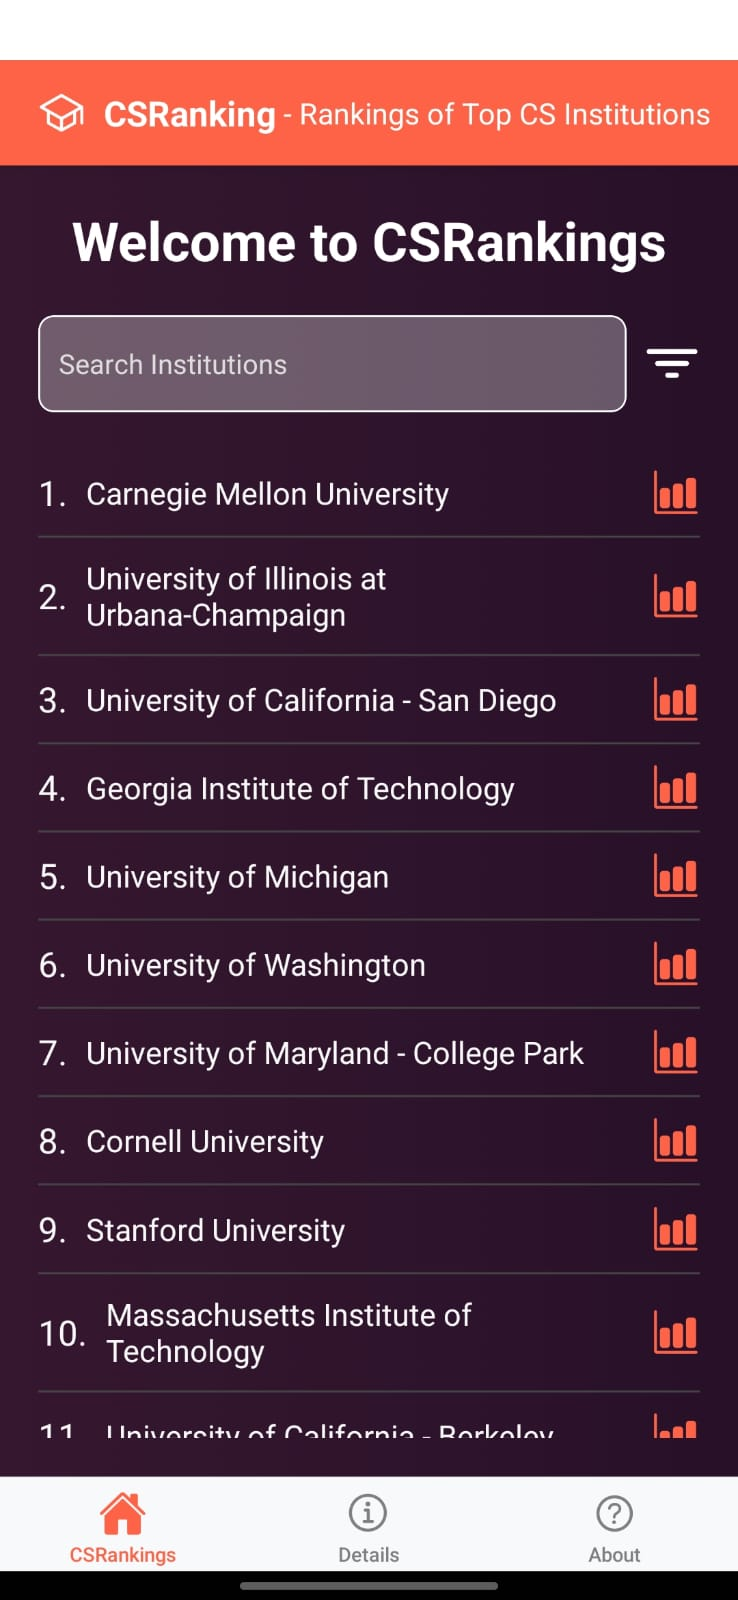
\includegraphics[width=0.3\textwidth, height=0.5\textheight]{home.jpg} % Adjust width and height as needed
    \caption{Navigator.}
    \label{fig:example_image}
\end{figure}

\subsubsection*{5.5.6 Styling and Theming}
\begin{itemize}
    \item Chose a consistent color scheme based on HEX code \texttt{\#33152d}.
    \item Designed responsive layouts for various screen sizes.
    \item Used \texttt{StyleSheet} to modularize and reuse styles across components.
\end{itemize}

\clearpage
\subsection*{5.6 Feature Highlights}

\subsubsection*{Interactive Features}
\begin{itemize}
    \item Dynamic search and filtering on the homepage.
    \item Interactive bar charts with data point click functionality.
\end{itemize}

\subsubsection*{Navigation}
\begin{itemize}
    \item Used \texttt{react-navigation} to implement stack navigation for multi-screen workflows.
\end{itemize}

\subsubsection*{Accessibility Enhancements}
\begin{itemize}
    \item Ensured touch targets were appropriately sized.
    \item Added labels and alt-text for accessibility compliance.
\end{itemize}

\subsubsection*{Responsive Design}
\begin{itemize}
    \item Tested on both Android and iOS to ensure consistent UI/UX.
\end{itemize}

\bigskip
\section*{6. Final Testing and Debugging}

Testing and debugging were critical steps in ensuring that the \texttt{CSRankings} app was reliable, user-friendly, and performed well across devices. The following methods were employed for manual testing, automated testing, and resolving bugs during the development process.

\subsubsection*{6.1 Manual Testing}

\textbf{Platforms Tested:}
\begin{itemize}
    \item The app was tested on Android simulators, iOS simulators, and a variety of physical devices with different screen sizes.
    \item Devices used for testing included:
    \begin{itemize}
        \item \textbf{Android:} Pixel 5, Samsung Galaxy S10.
        \item \textbf{iOS:} iPhone 12, iPhone SE.
    \end{itemize}
\end{itemize}

\textbf{Features Tested:}
\begin{itemize}
    \item \textbf{Navigation:}
    \begin{itemize}
        \item Ensured smooth transitions between tabs (Home, Details, About).
        \item Verified the Stack Navigator functionality for navigating from Home to Institution Details and Chart screens.
    \end{itemize}
    \item \textbf{Filters:}
    \begin{itemize}
        \item Tested \textit{``All Areas''} toggle to confirm it resets all sub-area selections.
        \item Verified that selected sub-areas dynamically filtered institutions.
    \end{itemize}
    \item \textbf{Chart Interactivity:}
    \begin{itemize}
        \item Checked the rendering of bar charts for institutions with varying numbers of publications.
        \item Confirmed that tapping on a chart bar displayed the correct publication details in an alert.
    \end{itemize}
    \item \textbf{Institution Detail Page:}
    \begin{itemize}
        \item Verified the accurate display of faculty information, including publication counts and external links.
        \item Tested external links (e.g., Google Scholar, DBLP) to ensure they opened in a web browser.
    \end{itemize}
    \item \textbf{UI Responsiveness:}
    \begin{itemize}
        \item Ensured proper layout and spacing for different screen resolutions.
        \item Checked the responsiveness of the search bar and tab navigation.
    \end{itemize}
\end{itemize}

\textbf{Edge Cases Tested:}
\begin{itemize}
    \item Institutions with no faculty data.
    \item Long institution names or sub-area titles.
    \item Empty search results.
    \item Rapid toggling of filters to ensure the app didn’t crash.
\end{itemize}

\textbf{Performance Checks:}
\begin{itemize}
    \item Verified that the app maintained a smooth scrolling experience even with a large dataset.
    \item Ensured minimal lag while navigating between screens and applying filters.
\end{itemize}

\subsubsection*{6.2 Automated Testing}

To ensure the robustness of the application, automated tests were implemented using \texttt{Jest} and \texttt{@testing-library/react-native}. The focus was on validating the functionality of core components, navigation, and edge case handling. Below is an overview of the testing framework and the specific tests conducted.

\clearpage
\bigskip
\textbf{Unit Testing Framework}
\begin{itemize}
    \item \textbf{Jest:} Used as the primary testing framework for its compatibility with React Native.
    \item \textbf{@testing-library/react-native:} Enabled testing of React Native components and their interactions.
\end{itemize}

\textbf{Tests Implemented}
\begin{enumerate}
    \item \textbf{HomeScreen Component}
    \begin{itemize}
        \item \textbf{Purpose:} To validate the homepage functionality and UI elements.
        \item \textbf{Tests Conducted:}
        \begin{itemize}
            \item Verified the rendering of the welcome message and search bar.
            \item Ensured the filter modal opened upon clicking the filter icon.
            \item Tested search functionality to filter institutions based on user input.
        \end{itemize}
    \end{itemize}

\begin{lstlisting}[language=JavaScript, caption={HomeScreen Tests}, label={lst:HomeScreen}]
import React from "react";
import { render, fireEvent } from "@testing-library/react-native";
import HomeScreen from "../HomeScreen";

describe("HomeScreen", () => {
  it("renders the welcome message", () => {
    const { getByText } = render(<HomeScreen navigation={{}} />);
    expect(getByText("Welcome to CSRankings")).toBeTruthy();
  });

  it("renders the search bar", () => {
    const { getByPlaceholderText } = render(<HomeScreen navigation={{}} />);
    expect(getByPlaceholderText("Search Institutions")).toBeTruthy();
  });

  it("opens filters modal when filter icon is pressed", () => {
    const { getByTestId, getByText } = render(<HomeScreen navigation={{}} />);
    const filterButton = getByTestId("filter-icon");
    fireEvent.press(filterButton);
    expect(getByText("Filter by Areas")).toBeTruthy();
  });
});
\end{lstlisting}

    \bigskip
    \item \textbf{ChartScreen Component}
    \begin{itemize}
        \item \textbf{Purpose:} To verify the proper rendering of charts and the functionality of chart interactions.
        \item \textbf{Tests Conducted:}
        \begin{itemize}
            \item Ensured the chart title and legend rendered correctly.
            \item Validated the click functionality on chart bars to display an alert with accurate details.
        \end{itemize}
    \end{itemize}

\begin{lstlisting}[language=JavaScript, caption={ChartScreen Tests}, label={lst:ChartScreen}]
import React from "react";
import { render, fireEvent } from "@testing-library/react-native";
import ChartScreen from "../ChartScreen";

const mockRoute = {
  params: {
    data: [5, 10, 15, 20],
    name: "Test Institution",
    categories: [
      {
        category_id: 1,
        category_name: "Category 1",
        sub_areas: [
          { sub_area_id: 1, name: "Area 1" },
          { sub_area_id: 2, name: "Area 2" },
          { sub_area_id: 3, name: "Area 3" },
          { sub_area_id: 4, name: "Area 4" },
        ],
      },
    ],
  },
};

describe("ChartScreen", () => {
  it("renders the chart title", () => {
    const { getByText } = render(<ChartScreen route={mockRoute} />);
    expect(getByText("Research Areas for Test Institution")).toBeTruthy();
  });

  it("renders the legend correctly", () => {
    const { getByText } = render(<ChartScreen route={mockRoute} />);
    expect(getByText("Area 1")).toBeTruthy();
    expect(getByText("Area 2")).toBeTruthy();
  });

  it("handles bar clicks correctly", () => {
    const { getByText } = render(<ChartScreen route={mockRoute} />);
    const bar = getByText("Area 1");
    fireEvent.press(bar);
    expect(getByText("Bar Clicked")).toBeTruthy();
  });
});
\end{lstlisting}

    \item \textbf{AboutScreen Component}
    \begin{itemize}
        \item \textbf{Purpose:} To validate the content rendering on the About screen, including links and titles.
        \item \textbf{Tests Conducted:}
        \begin{itemize}
            \item Verified the correct rendering of the \textit{``About CSRankings''} title.
            \item Ensured all external links and text content were visible.
        \end{itemize}
    \end{itemize}

\begin{lstlisting}[language=JavaScript, caption={AboutScreen Tests}, label={lst:AboutScreen}]
import React from "react";
import { render } from "@testing-library/react-native";
import AboutScreen from "../AboutScreen";

describe("AboutScreen", () => {
  it("renders the about title", () => {
    const { getByText } = render(<AboutScreen />);
    expect(getByText("About CSRankings")).toBeTruthy();
  });

  it("renders the video link", () => {
    const { getByText } = render(<AboutScreen />);
    expect(getByText("Click the image above to watch the introduction video on YouTube.")).toBeTruthy();
  });

  it("renders external links correctly", () => {
    const { getByText } = render(<AboutScreen />);
    expect(getByText("https://github.com/emeryberger/CSRankings")).toBeTruthy();
  });
});
\end{lstlisting}

\end{enumerate}

\begin{figure}[H]
    \centering
    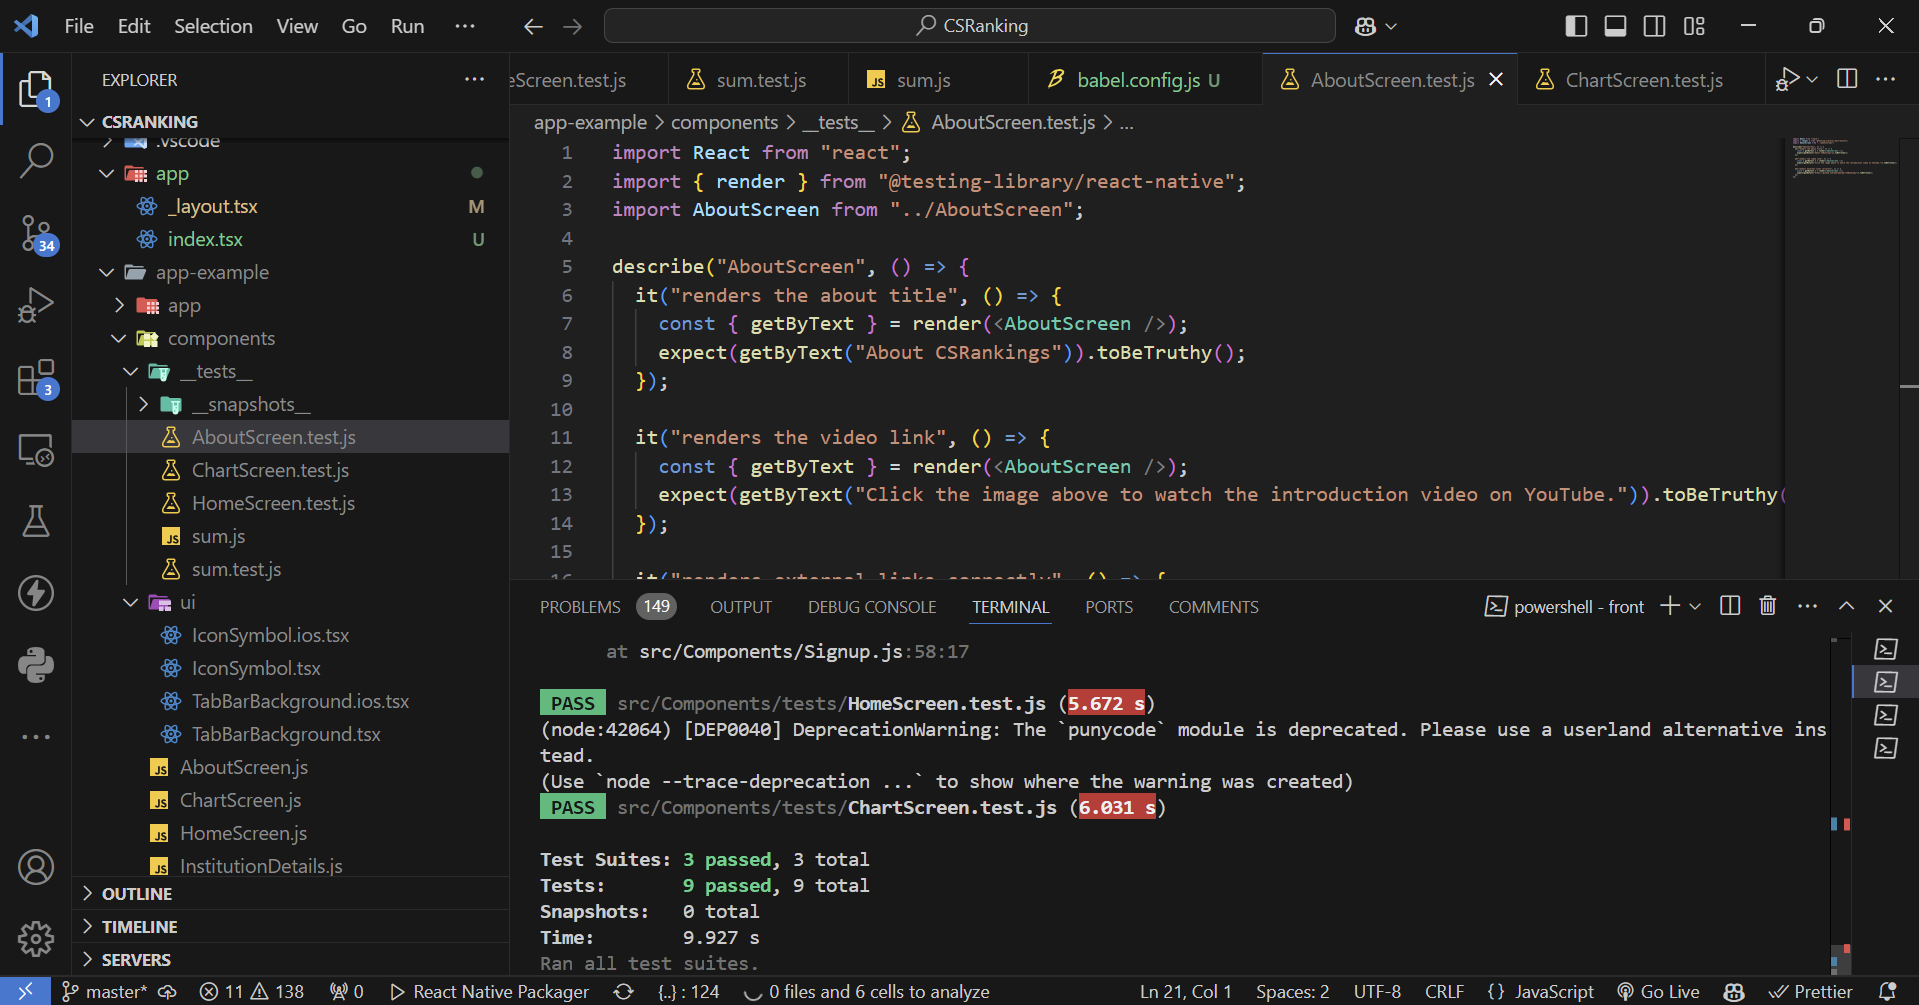
\includegraphics[width=1\textwidth, height=0.5\textheight]{testcases.png} % Adjust width and height as needed
    \caption{Test Cases.}
    \label{fig:example_image}
\end{figure}

\setcounter{section}{6} % Set the section counter to 6 so the next section is numbered 7

\section{Challenges and Assumptions}

\subsection{Challenges}

\begin{itemize}
    \item \textbf{Understanding the Website's Structure:} 
    Without the ability to ask questions, reverse-engineering the hierarchy and functionality of the original website was challenging. I relied on closely analyzing the website's behavior and data presentation to make accurate assumptions.
    
    \item \textbf{SDK Compatibility Issues:}
    Midway through the project, Expo SDK 51 faced compatibility issues with several dependencies. This required updating the project to SDK version 52. I resolved this by running the installation with the \texttt{@latest} flag, which ensured all dependencies were updated to versions compatible with the latest Expo SDK.
    
    \item \textbf{Dynamic State Management:}
    Managing dynamic states for filters and charts presented challenges in ensuring real-time updates while maintaining performance. React's \texttt{useState} and \texttt{useEffect} hooks were extensively optimized to handle the complex dependencies.
    
    \item \textbf{Chart Interactivity:}
    Implementing interactive charts required additional attention to handle tap events accurately, especially for small screens. Adjusting bar spacing and scaling dynamically improved usability.
    
    \item \textbf{Data Integration:}
    Merging multiple static JSON files to simulate backend behavior was tricky. I ensured that the linked data between institutions, faculty, and publication areas was robust and error-free.
    
    \item \textbf{UI Responsiveness:}
    Designing the UI to maintain consistent layouts across various screen sizes and orientations required careful styling adjustments using Flexbox and percentage-based dimensions.
\end{itemize}

\subsection{Assumptions}

\begin{itemize}
    \item \textbf{Hardcoded Data:}
    As backend integration was outside the scope of this project, I assumed that all research areas, institutions, and publication data could be hardcoded into JSON files.
    
    \item \textbf{Core Functionality:}
    The focus was primarily on replicating the main features of the website, such as rankings, filters, and charts, rather than implementing advanced backend features or additional enhancements.
\end{itemize}

\bigskip
\section{Platform Compatibility Testing}

\subsection{Android Compatibility}
\begin{itemize}
    \item Verified the application on Android simulators and physical devices.
    \item Tested navigation, filters, and charts on various Android screen sizes.
    \item Ensured responsiveness and performance remained optimal, even on older devices.
\end{itemize}

\subsection{iOS Compatibility}
\begin{itemize}
    \item Tested the app on iOS simulators and devices such as iPhone 11 and iPhone 14.
    \item Verified smooth transitions between screens and chart interactivity.
    \item Checked compatibility with iOS-specific behaviors like swipe gestures and safe areas.
\end{itemize}

\subsection{Cross-Platform Testing}
\begin{itemize}
    \item Ensured the app adhered to platform-specific design guidelines while maintaining consistent functionality.
    \item Adjusted navigation and modal styles to align with Android's Material Design and iOS's Human Interface Guidelines.
    \item Validated the use of React Native's platform-specific APIs to ensure seamless behavior on both platforms.
\end{itemize}

\begin{figure}[H]
    \centering
    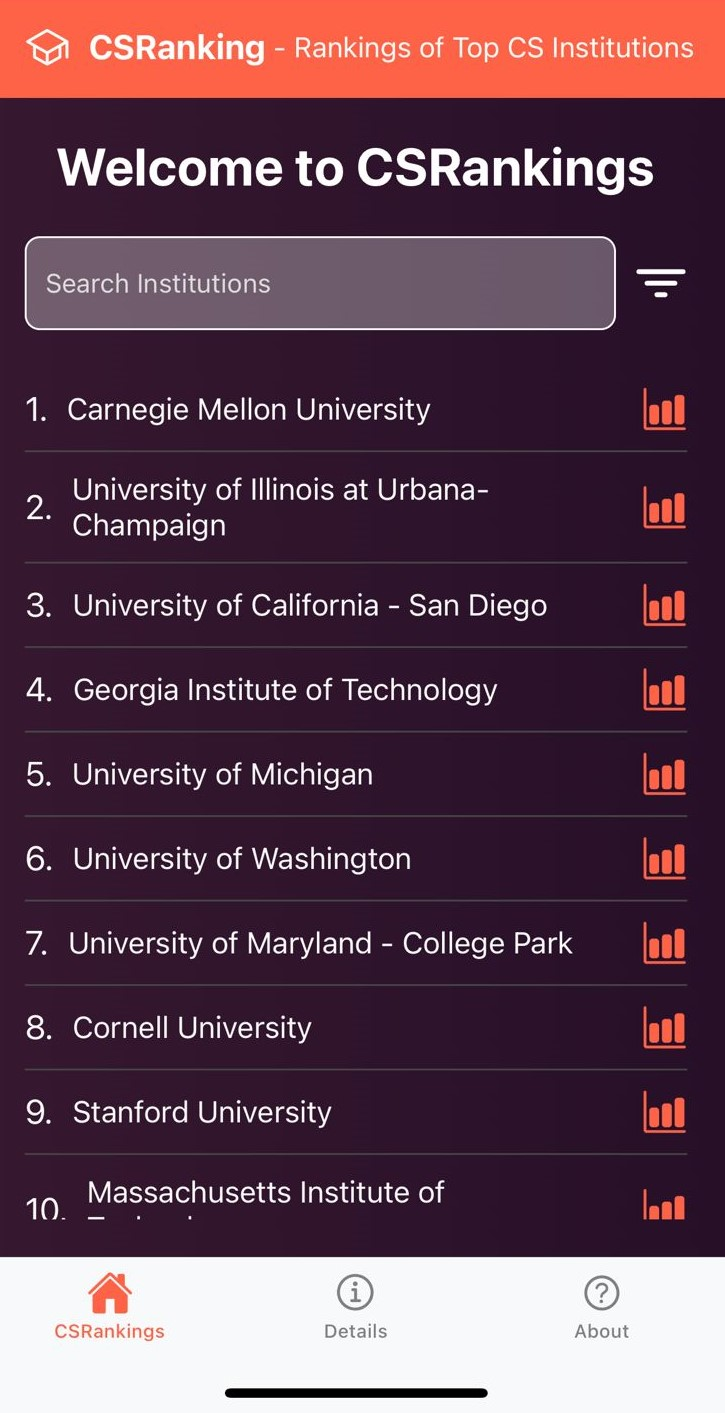
\includegraphics[width=0.3\textwidth, height=0.5\textheight]{homeios.jpeg} % Adjust width and height as needed
    \caption{CSRanking app on IOS.}
    \label{fig:example_image}
\end{figure}

\begin{figure}[H]
    \centering
    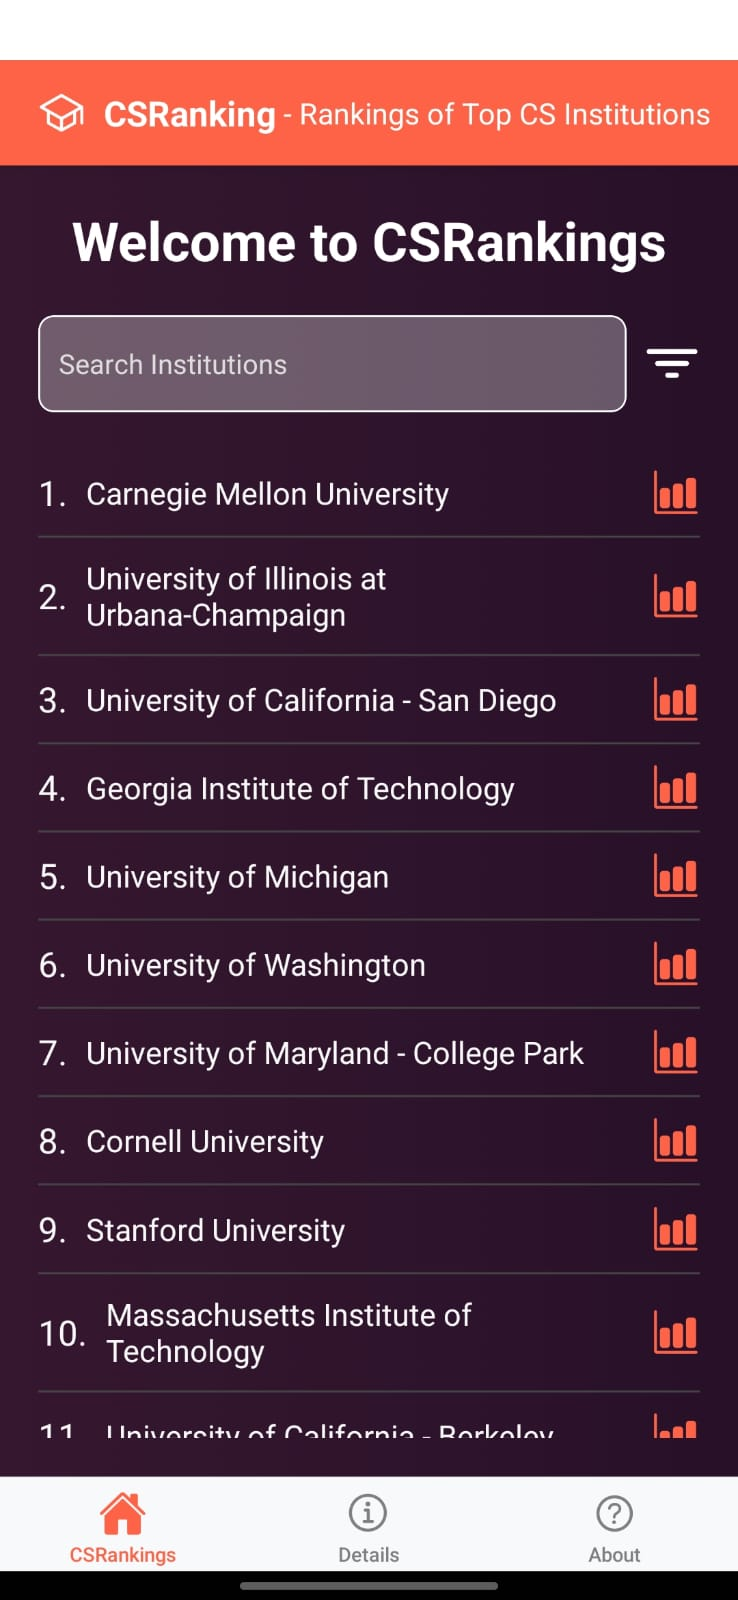
\includegraphics[width=0.3\textwidth, height=0.5\textheight]{home.jpg} % Adjust width and height as needed
    \caption{CSRankingAPP on Android.}
    \label{fig:example_image}
\end{figure}

\section{Conclusion and Future Enhancements}

\subsection{Conclusion}

The \texttt{CSRankings} app successfully replicates the core functionality of the website in a mobile-friendly manner. The project demonstrates a robust understanding of React Native, state management, and dynamic UI/UX development.

\bigskip
\subsection{Future Enhancements}

\begin{itemize}
    \item Adding real-time backend integration to fetch live data.
    \item Including additional interactive visualizations (e.g., pie charts).
    \item Enhancing filters with multi-select and search options.
    \item Improving accessibility features, such as voice commands and larger text support.
\end{itemize}

\section{Disclosure of AI Tool Usage}

LLMs like ChatGPT were instrumental in developing the \texttt{CSRankings} Mobile App by assisting with:

\begin{itemize}
    \item \textbf{Styling:} Suggested color schemes, typography, and responsive UI layouts to enhance cross-platform usability.
    \item \textbf{Logic Development:} Provided optimized solutions for managing dynamic filters, charts, and data integration using React hooks.
    \item \textbf{Debugging:} Helped resolve layout issues, SDK compatibility challenges, and state management bugs.
    \item \textbf{Report Writing:} Structured and articulated the project report, including challenges, solutions, and technical implementations.
    \item \textbf{Code Quality:} Guided best practices for React Native, modularization, and writing unit tests with Jest.
\end{itemize}

\section{GitHub Repository}

The project can be accessed at the following link: \url{https://github.com/rmusukudabbidi/CSRanking}







 
% --------------------------------------------------------------
%     You don't have to mess with anything below this line.
% --------------------------------------------------------------
 
\end{document}
